%% pdfo.tex
%% Copyright 2023 Tom M. Ragonneau and Zaikun Zhang
\RequirePackage{fix-cm}
\documentclass[
    smallextended,  % one column (second format)
    %draft,          % to make overfull boxes visible
    final,        % the opposite of draft
    % referee,      % required to produce a hardcopy for the referee with a special layout (bigger interline spacing)
]{svjour3}
%
%\usepackage{mathptmx}   % PostScript Times fonts (they may not look quite natural).
%
\usepackage{amsfonts}
\usepackage{amsmath}
\usepackage{amssymb}
\usepackage{booktabs}
\usepackage{caption}
\usepackage[acronym]{glossaries-extra}
\usepackage{graphicx}
\usepackage{ifthen}
\usepackage[final]{listings}
\usepackage{lstautogobble}
\usepackage{siunitx}
\usepackage{subcaption}
\usepackage{url}
\usepackage{xargs}
% Get back the upright capital Greek letters
\DeclareMathSymbol{\Gamma}{\mathalpha}{operators}{"00}
\DeclareMathSymbol{\Delta}{\mathalpha}{operators}{"01}
\DeclareMathSymbol{\Theta}{\mathalpha}{operators}{"02}
\DeclareMathSymbol{\Lambda}{\mathalpha}{operators}{"03}
\DeclareMathSymbol{\Xi}{\mathalpha}{operators}{"04}
\DeclareMathSymbol{\Pi}{\mathalpha}{operators}{"05}
\DeclareMathSymbol{\Sigma}{\mathalpha}{operators}{"06}
\DeclareMathSymbol{\Upsilon}{\mathalpha}{operators}{"07}
\DeclareMathSymbol{\Phi}{\mathalpha}{operators}{"08}
\DeclareMathSymbol{\Psi}{\mathalpha}{operators}{"09}
\DeclareMathSymbol{\Omega}{\mathalpha}{operators}{"0A}
%
\DeclareMathOperator*\argmin{arg\,min}
\DeclareMathOperator\range{\mathcal{R}}
\DeclareMathOperator\rank{rank}
\newcommand{\C}{\mathbb{C}}
\newcommand{\F}{\mathbb{F}}
\newcommand{\N}{\mathbb{N}}
\newcommand{\NN}{\mathrm{N}}
\newcommand{\Q}{\mathbb{Q}}
\newcommand{\R}{\mathbb{R}}
\newcommand{\T}{\mathsf{T}}
\newcommand{\Z}{\mathbb{Z}}
\newcommand{\abs}[2][]{#1\lvert#2#1\rvert}
\newcommand{\aeq}{A_{\scriptscriptstyle\mathcal{E}}}
\newcommand{\aub}{A_{\scriptscriptstyle\mathcal{I}}}
\newcommand{\base}{{\text{b}}}
\newcommand{\beq}{b_{\scriptscriptstyle\mathcal{E}}}
\newcommand{\bub}{b_{\scriptscriptstyle\mathcal{I}}}
\newcommand{\ceil}[2][]{#1\lceil#2#1\rceil}
\newcommand{\ceq}{\con[\scriptscriptstyle\mathcal{E}]}
\newcommand{\con}[1][i]{c\ifthenelse{\equal{#1}{}}{}{_{#1}}}
\newcommand{\cub}{\con[\scriptscriptstyle\mathcal{I}]}
\newcommand{\drop}{{\text{d}}}
\newcommand{\du}{\mathrm{d}}
\newcommand{\eqdef}{\mathrel{\stackrel{\mathsf{def}}{=}}}
\newcommand{\eu}{\mathrm{e}}
\newcommand{\floor}[2][]{#1\lfloor#2#1\rfloor}
\newcommand{\frob}{\mathsf{F}}
\newcommand{\fsetm}[1][k]{\Omega_{#1}}
\newcommand{\fset}{\Omega}
\newcommand{\func}{\mathcal{F}}
\newcommand{\geo}{{\text{g}}}
\newcommand{\grad}[1][k]{g\ifthenelse{\equal{#1}{}}{}{_{#1}}}
\newcommand{\hess}[1][k]{B\ifthenelse{\equal{#1}{}}{}{_{#1}}}
\newcommand{\inner}[2][]{#1\langle#2#1\rangle}
\newcommand{\iter}[1][k]{x\ifthenelse{\equal{#1}{}}{}{_{#1}}}
\newcommand{\iu}{\mathrm{i}}
\newcommand{\negp}[2][]{#1[#2#1]_-}
\newcommand{\norm}[2][]{#1\lVert#2#1\rVert}
\newcommand{\objm}[1][k]{\obj\ifthenelse{\equal{#1}{}}{}{_{#1}}}
\newcommand{\obj}{f}
\newcommand{\posp}[2][]{#1[#2#1]_+}
\newcommand{\qspace}[1][n]{\mathcal{Q}\ifthenelse{\equal{#1}{}}{}{_{#1}}}
\newcommand{\radalt}[1][k]{\bar{\Delta}\ifthenelse{\equal{#1}{}}{}{_{#1}}}
\newcommand{\rad}[1][k]{\Delta\ifthenelse{\equal{#1}{}}{}{_{#1}}}
\newcommand{\radlb}[1][k]{\rho\ifthenelse{\equal{#1}{}}{}{_{#1}}}
\newcommand{\set}[2][]{#1\{#2#1\}}
\newcommand{\st}{\text{s.t.}}
\newcommand{\trust}{{\text{t}}}
\newcommand{\xl}{l}
\newcommand{\xpt}[1][k]{\mathcal{Y}\ifthenelse{\equal{#1}{}}{}{_{#1}}}
\newcommand{\xu}{u}
\newcommandx{\conm}[2][1=k,2=i]{c_{#1, #2}}
%
\glsdisablehyper
\newabbreviation{auc}{AUC}{area under the curve}
\newabbreviation{dfo}{DFO}{derivative-free optimization}
\newabbreviation{psb}{PSB}{Powell's symmetric Broyden}
\newabbreviation{rbf}{RBF}{radial basis function}
\newabbreviation{roc}{ROC}{receiver operating characteristic}
\newabbreviation{rs}{RS}{Random Search}
\newabbreviation{svm}{SVM}{support vector machine}
\newabbreviation{tpe}{TPE}{Tree-Structured Parzen Estimator}
\newacronym{bobyqa}{BOBYQA}{Bound Optimization BY Quadratic Approximation}
\newacronym{bfgs}{BFGS}{Broyden-Fletcher-Goldfarb-Shanno}
\newacronym{cg}{CG}{Conjugate Gradient}
\newacronym{cobyla}{COBYLA}{Constrained Optimization BY Linear Approximations}
\newacronym{cobyqa}{COBYQA}{Constrained Optimization BY Quadratic Approximations}
\newacronym{lincoa}{LINCOA}{LINearly Constrained Optimization Algorithm}
\newacronym{newuoa}{NEWUOA}{NEW Unconstrained Optimization Algorithm}
\newacronym{pdfo}{PDFO}{Powell's Derivative-Free Optimization solvers}
\newacronym{uobyqa}{UOBYQA}{Unconstrained Optimization BY Quadratic Approximation}
%
\graphicspath{{figures/}}
%
\lstset{
    autogobble=true,
    basicstyle=\normalsize\ttfamily,
    belowcaptionskip=\bigskipamount,
    breakautoindent=true,
    breakatwhitespace=false,
    breaklines=true,
    commentstyle=\itshape\color{black!50},
    frame=tb,
    keywordstyle=\bfseries,
    postbreak=\space,
    showstringspaces=false,
    stepnumber=1,
    stringstyle=\itshape,
    tabsize=4,
}
\lstnewenvironment{matlablst}[1][]{
    \lstset{
        language=matlab,
        % morekeywords={},
        #1,
    }
}{}
%
\sisetup{
    group-minimum-digits=4,
    group-separator={,},
}
%
\input{ushyphex}    % hyphenation exceptions for US English

%
%\usepackage[final]{microtype}
%\usepackage[nobottomtitles*]{titlesec}  % no section title at the bottom of pages
% N.B. titlesec changes the behavior of ``\paragraph'', adding a line break.
\interfootnotelinepenalty=10000  % prevent footnote from running to the next page
% no line break in inline math
\interdisplaylinepenalty=10000
\relpenalty=10000
\binoppenalty=10000
% no widow or orphan lines
\clubpenalty=10000
\widowpenalty=10000
\displaywidowpenalty=10000
\usepackage{xspace}

% Cross-referencing and colorization
\usepackage[final,hyperfootnotes=false]{hyperref}
\usepackage[dvipsnames]{xcolor}
\usepackage{url}
\hypersetup{
    colorlinks=true,
    linkcolor=OliveGreen,
    anchorcolor=black,
    citecolor=MidnightBlue,
    filecolor=black,
    menucolor=black,
    runcolor=black,
    urlcolor=black,
}
\newcommand{\red}{\textcolor{red}}
\newcommand{\kkt}{KKT\xspace}
\newcommand{\hugefun}{\texttt{HUGEFUN}\xspace}
\newcommand{\pdfofun}{\texttt{pdfo}\xspace}
\newcommand{\cobylafun}{\texttt{cobyla}\xspace}
\newcommand{\uobyqafun}{\texttt{uobyqa}\xspace}
\newcommand{\newuoafun}{\texttt{newuoa}\xspace}
\newcommand{\bobyqafun}{\texttt{bobyqa}\xspace}
\newcommand{\lincoafun}{\texttt{lincoa}\xspace}
\renewcommand{\baselinestretch}{1.1}

%
\journalname{Mathematical Programming Computation}
\title{PDFO --- A Cross-Platform Package for Powell's Derivative-Free Optimization Solvers}
\subtitle{}
\titlerunning{PDFO}
\dedication{To the memory of late Prof.\ M. J. D. Powell FRS}
\author{Tom M. Ragonneau \and Zaikun Zhang}
\authorrunning{}
\institute{%
    T. M. Ragonneau \at
        Department of Applied Mathematics, The Hong Kong Polytechnic University, Hong Kong\\
        ORCID: 0000-0003-2717-2876\\
        \email{tom.ragonneau@polyu.edu.hk}
    \and
    Z. Zhang (corresponding author)\at
        Department of Applied Mathematics, The Hong Kong Polytechnic University, Hong Kong\\
        ORCID: 0000-0001-8934-8190\\
        \email{zaikun.zhang@polyu.edu.hk}
}
\date{Received: date / Accepted: date}
%
\begin{document}

\maketitle

\begin{abstract}
    Late Professor M. J. D. Powell designed five derivative-free optimization methods, namely \gls{cobyla}, \gls{uobyqa}, \gls{newuoa}, \gls{bobyqa}, and \gls{lincoa}.
    The algorithms were implemented in Fortran 77 and may not be easily accessible to some users.
    This paper introduces the~\gls{pdfo}~(\glsxtrlong{pdfo}) package, which provides user-friendly Python and MATLAB interfaces to Powell's code.
    %, and has been downloaded more than \num{50000} times as of February 2023 (mirror downloads excluded).
    With~\gls{pdfo}, users can call each of Powell's algorithms directly based on their own choice.
    Alternatively, if the user does not specify any algorithm, the package can also select one automatically based on the problem characteristics.
    % When a problem can be solved by multiple algorithms (for example, an unconstrained problem can be solved by all five algorithms), the selection is made based on experimental results on the CUTEst problems.
    We also provide an overview on Powell's methods and share some observations on these methods based on experiments conducted using~\gls{pdfo}.

    \keywords{Derivative-free optimization \and model-based methods \and COBYLA \and UOBYQA \and NEWUOA \and
    BOBYQA \and LINCOA}
    \subclass{65K05 \and 90C30 \and 90C56 \and 90-04}
    %\CRclass{CR code1 \and CR code2 \and more}
\end{abstract}

\section{Introduction}

Most optimization algorithms rely on classical or generalized derivative information of the objective and constraint functions.
However, in many applications, such information is not available.
This is the case, for example, if the objective function does not have an explicit formulation but can only be evaluated through complex simulations or experiments.
Optimization problems of such kind arise from automatic error analysis~\cite{Higham_1993,Higham_2002}, machine learning~\cite{Ghanbari_Scheinberg_2017}, analog circuit design~\cite{Latorre_Etal_2019}, aircraft engineering~\cite{Gazaix_Etal_2019}, and chemical product design~\cite{Sun_Etal_2020}, to name but a few.
These problems motivate the development of optimization algorithms that use only function values but not derivatives, also known as \gls{dfo} algorithms.

Powell developed five algorithms to tackle unconstrained and constrained problems without using derivatives, namely~\gls{cobyla}~\cite{Powell_1994}, \gls{uobyqa}~\cite{Powell_2002}, \gls{newuoa}~\cite{Powell_2006}, \gls{bobyqa}~\cite{Powell_2009}, and \gls{lincoa}.
He did not only propose these algorithms but also implemented them into publicly available solvers, paying great attention to the stability and complexity of their numerical linear algebra computations.
Renowned for their robustness and efficiency, these solvers are used in a wide spectrum of applications, for instance, aeronautical engineering~\cite{Gallard_Etal_2018}, astronomy~\cite{Biviano_Etal_2013,Mamon_Biviano_Boue_2013}, computer vision~\cite{Izadinia_Shan_Seitz_2017}, robotics~\cite{Mombaur_Truong_Laumond_2010}, and statistics~\cite{Bates_Etal_2015}.

However, Powell coded the solvers in Fortran 77, an old-fashion language that damps the enthusiasm of many users to exploit these solvers in their projects.
There has been considerable demand from both researchers and practitioners for the availability of Powell's solvers in more user-friendly languages such as Python and MATLAB.
Our aim is to wrap Powell's Fortran code into a package named \gls{pdfo}, which enables users of such languages to call Powell's solvers without any need to deal with the Fortran code.
For each supported language, \gls{pdfo} provides a simple function that can invoke one of Powell's solvers according to the user's request (if any) or according to the type of the problem to solve.
The current release (Version 1.2) of \gls{pdfo} supports Python and MATLAB, with more languages to be covered in the future.
The signature of the Python subroutine is consistent with the \texttt{minimize} function of the SciPy optimization library; the signature of the MATLAB subroutine is consistent with the \texttt{fmincon} function of the MATLAB Optimization Toolbox.
\gls{pdfo} is cross-platform, and available on Linux, macOS, and Windows at
\begin{center}
    \url{https://www.pdfo.net/}.
\end{center}
It has been downloaded more than \num{50000} times as of February 2023 (mirror downloads excluded).
Moreover, it is one of the optimization engines in GEMSEO~\cite{Gallard_Etal_2018},
an industrial software package for Multidisciplinary Design Optimization (MDO).

\Gls{pdfo} is not the first attempt to facilitate the usage of Powell's solvers in languages other than Fortran.
Various efforts have been made in this direction.
Py-BOBYQA~\cite{Cartis_Etal_2019,Cartis_Roberts_Sheridan-Methven_2022} provides a Python implementation of \gls{bobyqa}; NLopt~\cite{Johnson_2019} includes multi-language interfaces for \gls{cobyla}, \gls{newuoa}, and \gls{bobyqa}; minqa~\cite{Bates_Etal_2014} wraps \gls{uobyqa}, \gls{newuoa}, and \gls{bobyqa} in R; SciPy~\cite{Virtanen_Etal_2020} makes \gls{cobyla} available in Python under its optimization library.
However, \gls{pdfo} has several features that distinguishes itself from others.

\begin{enumerate}
    \item \emph{Comprehensiveness.}
    To the best of our knowledge, \gls{pdfo} is the only package that provides all of \gls{cobyla},
    \gls{uobyqa}, \gls{newuoa}, \gls{bobyqa}, and \gls{lincoa} with a \emph{uniform interface}.
    %In addition to homogenizing the usage, such an interface eases the comparison between these solvers in case multiple of them are able to tackle a given problem.
    %By doing so, we may gain insights that cannot be obtained otherwise into the behavior of the solvers.
    %, as will be illustrated in~\cref{sec:fake}.

    \item \emph{Solver selection.}
    %When using \gls{pdfo}, the user can specifically call one of Powell's solvers. If the user does not specify any solver,
    \gls{pdfo} can automatically select a solver for a given problem.
    The selection takes into consideration the performance of the solvers on the CUTEst~\cite{Gould_Orban_Toint_2015} problem set.
    %Interestingly, it turns out that the solver with the best performance may not be the most intuitive one.
    %For example, \gls{newuoa} is not always the best choice for solving an unconstrained problem.

    \item \emph{Problem preprocessing.}
    \Gls{pdfo} preprocesses the inputs to simplify the problem and reformulate it to meet the requirements of Powell's solvers.
    %For instance, if the problem has linear constraints~$\aeq x = \beq$, \gls{pdfo} rewrites it into a problem on the null space of~$\aeq$, eliminating such constraints and reducing the problem's dimension.
    %As another example, the starting point of a linearly constrained problem is projected onto the feasible region, because \gls{lincoa} needs a feasible starting point to work properly.

    \item \emph{Code patching.}
        \gls{pdfo} patches several bugs in the Fortran code.
        Such bugs can lead to serious problems such as infinite cycling or memory errors.
    %During the development of \gls{pdfo}, we spotted some bugs in the original Fortran code, which led to infinite cycling or segmentation faults on ill-conditioned problems.
    %The bugs have been patched in \gls{pdfo}.
    %We also provide an option that can enforce the package to use the original code of Powell without the patches, which is not recommended except for research.
    %In addition, \gls{pdfo} provides \gls{cobyla} in double precision, whereas Powell used single precision when he implemented it in the 1990s.

    \item \emph{Fault tolerance.}
    \Gls{pdfo} tolerates failures of function evaluations when NaN values are returned.
    In case of such failures, \gls{pdfo} will not exit but try to progress.
    %Moreover, \gls{pdfo} ensures that the returned solution is not a point where the evaluation
    %fails, while the original code of Powell may return a point whose objective function value is numerically~NaN.

    \item \emph{Additional options.}
    \Gls{pdfo} includes options for the user to control the solvers in some manners that are useful in practice.
    For example, the user can request \gls{pdfo} to scale the problem according to bound constraints on the variables before solving~it.
\end{enumerate}

\red{
The remaining part of this paper is organized as follows.
Section~\ref{sec:dfo} briefly reviews \gls{dfo} methods, in order to provide the context of Powell's algorithms.
We then present an overview of Powell's \gls{dfo} algorithms in Section~\ref{sec:powell}.
A detailed exposition of~\gls{pdfo} is given in Section~\ref{sec:pdfo}.
Section~\ref{sec:numerical} shows some numerical experiments conducted using~\gls{pdfo}.
We conclude the paper with some remarks in Section~\ref{sec:conclude}.
}

\section{A brief review of \glsfmtshort{dfo} methods}
\label{sec:dfo}

Consider a nonlinear optimization problem
\begin{equation}
    \label{eq:nlc}
    \min_{x \in \fset} \obj(x),
\end{equation}
where~$\obj : \R^n \to \R$ is the objective function and~$\fset \subseteq \R^n$ represents the feasible region.
As summarized in~\cite{Conn_Scheinberg_Vicente_2009b}, two strategies have been developed to tackle
the problem~\eqref{eq:nlc} without using derivatives, which we will introduce in the following.

The first strategy, known as direct search\footnote{In some early papers (e.g.,~\cite{Powell_1994,Powell_1998}),
Powell and many other authors used ``direct search'' to mean what is known as ``\glsfmtlong{dfo}'' today. Powell rarely used the word ``derivative-free optimization.''
The only exceptions known to us are his last paper~\cite{Powell_2015} and his distinguished lecture
titled ``A parsimonious way of constructing quadratic models from values of the objective function in
derivative-free optimization'' at the National Center for Mathematics and Interdisciplinary Sciences,
Beijing on November 4, 2011~\cite{Buhmann_Fletcher_Iserles_Toint_2018}.}, explores the objective function~$\obj$ and chooses iterates by simple comparisons of function values, examples including the Nelder-Mead algorithm~\cite{Nelder_Mead_1965}, the MADS methods~\cite{Audet_Dennis_2006,Abramson_Audet_2006,Digabel_2011}, and BFO~\cite{Porcelli_Toint_2017,Porcelli_Toint_2020,Porcelli_Toint_2022}.
See~\cite{Kolda_Lewis_Torczon_2003},~\cite[Chapters~7 and~8]{Conn_Scheinberg_Vicente_2009b},~\cite[Part~3]{Audet_Hare_2017}, and~\cite[\S~2.1]{Larson_Menickelly_Wild_2019} for more discussions on this paradigm, and we refer to~\cite{Gratton_Etal_2015,Gratton_Etal_2019} for recent developments on randomized methods in this category.

The second strategy approximates the original problem~\eqref{eq:nlc} by relatively simple models and locates the iterates according to these models.
Algorithms with this strategy are referred to as model-based methods. They often make use of the models within a trust-region framework~\cite{Conn_Gould_Toint_2000,Conn_Scheinberg_Vicente_2009a,Yuan_2015} or a line-search framework~\cite{Berahas_Byrd_Nocedal_2019,Shi_Etal_2022}.
Interpolation and regression are two common ways of establishing the models~\cite{Powell_2001,Conn_Scheinberg_Vicente_2008a,Conn_Scheinberg_Vicente_2008b,Wild_Regis_Shoemaker_2008,Bandeira_Scheinberg_Vicente_2012,Billups_Larson_Graf_2013,Regis_Wild_2017}.
Algorithms using finite-difference approximations of gradients can also be regarded as model-based
methods, because such approximations essentially come from linear (for forward and backward finite
differences) or quadratic (for central finite difference) interpolation of the function under
consideration over rather special interpolation sets~(see~\cite[\S~1.4.3]{Ragonneau_2022} for more comments).
Most model-based \gls{dfo} methods employ polynomial models that are linear or quadratic, examples including
Powell's algorithms~\cite{Powell_1994,Powell_2002,Powell_2006,Powell_2009} in \gls{pdfo},
MNH~\cite{Wild_2008}, DFLS~\cite{Zhang_Conn_Scheinberg_2010},
DFO-TR~\cite{Bandeira_Scheinberg_Vicente_2012}, and DFO-LS~\cite{Cartis_Etal_2019,Hough_Roberts_2022}, but there are also successful cases exploiting \glspl{rbf}, such as ORBIT~\cite{Wild_Regis_Shoemaker_2008}, CONORBIT~\cite{Regis_Wild_2017}, and BOOSTERS~\cite{Oeuvray_Bierlaire_2009}.
%Model-based \gls{dfo} is one of the motivations for studying trust-region and line-search methods with randomized models, for which we refer to~\cite{Bandeira_Scheinberg_Vicente_2014,Gratton_Etal_2018,Cartis_Scheinberg_2018} as examples.

Hybrids between direct-search and model-based approaches exist, for example~\cite{Custodio_Vicente_2007}, Implicit Filtering~\cite[Algorithm~4.7]{Kelley_2011}, and~\cite{Conn_Digabel_2013}.
Theory of global convergence and convergence rate has been established for both direct-search and model-based methods~\cite{Torczon_1997,Conn_Scheinberg_Toint_1997a,Kolda_Lewis_Torczon_2003,Conn_Scheinberg_Vicente_2009a,Powell_2012,Vicente_2013,Dodangeh_Vicente_2016,Garmanjani_Judice_Vicente_2016,Gratton_Royer_Vicente_2020}.
It is worth noting that the performance of \gls{dfo} algorithms is measured in general by the number of function evaluations needed for solving a given problem, as the objective and constraint functions in \gls{dfo} problems are commonly
expensive to evaluate.
Therefore, the worst-case complexity in terms of function evaluations is a major theoretical aspect of \gls{dfo} algorithms.
Examples of such complexity analysis can be found in~\cite{Vicente_2013,Gratton_Etal_2015,Dodangeh_Vicente_2016,Dodangeh_Vicente_Zhang_2016}.
For more extensive discussions on \gls{dfo} methods and theory, see the monographs~\cite{Conn_Scheinberg_Vicente_2009b,Audet_Hare_2017}, the survey
papers~\cite{Rios_Sahinidis_2013,Custodio_Scheinberg_Vicente_2017,Larson_Menickelly_Wild_2019}, the recent thesis~\cite{Ragonneau_2022}, and the references therein.

\section{Powell's derivative-free algorithms}
\label{sec:powell}

Powell published in 1964 his first \gls{dfo} algorithm based on conjugate directions~\cite{Powell_1964}\footnote{According to Google Scholar, this is Powell's second published paper and also the second most cited work.
The earliest and meanwhile most cited one is his paper on the DFP method~\cite{Fletcher_Powell_1963},
co-authored with Fletcher and published in 1963. DFP is not a DFO algorithm but the first
quasi-Newton method. The least-change property~\cite{Dennis_Schnabel_1979} of quasi-Newton methods
is a major motivation for Powell to investigate the least Frobenius norm updating~\cite{Powell_2004b}
of quadratic models in DFO, which is the backbone of \gls{newuoa}, \gls{bobyqa}, and \gls{lincoa}.}.
His code for this algorithm is contained in the HSL Mathematical Software Library~\cite{HSL} as subroutine \texttt{VA24}.
It is not included in \gls{pdfo} because the code is not in the public domain, although open-source implementations are available~(see~\cite[footnote~4]{Conn_Scheinberg_Toint_1997b}).

From the 1990s to the final days of his career, Powell developed five model-based \gls{dfo}
algorithms to solve~\eqref{eq:nlc}, namely \gls{cobyla}~\cite{Powell_1994}~(for nonlinearly
constrained problems), \gls{uobyqa}~\cite{Powell_2002}~(for unconstrained problems),
\gls{newuoa}~\cite{Powell_2006}~(for unconstrained problems), \gls{bobyqa}~\cite{Powell_2009}~(for
bound-constrained problems), and \gls{lincoa} (for linearly constrained problems).
Moreover, Powell implemented these algorithms into Fortran solvers and made the code publicly available.
They are the cornerstones of \gls{pdfo}.
This section provides an overview of these five algorithms, starting with a sketch in
Section~\ref{ssec:sketch} and then presenting more details afterwards.

\subsection{A sketch of the algorithms}
\label{ssec:sketch}

Powell's model-based \gls{dfo} algorithms are trust-region methods.
At iteration~$k$, the algorithms construct a linear (for \gls{cobyla}) or quadratic (for the other methods) model~$\objm$ for the objective function~$f$ to meet the interpolation condition
\begin{equation}
    \label{eq:itpls}
    \objm(y) = \obj(y), \quad y \in \xpt,
\end{equation}
where~$\xpt \subseteq \R^n$ is a finite interpolation set updated along the iterations.
\Gls{cobyla} models the constraints by linear interpolants on~$\xpt$ as well.
Instead of repeating Powell's description of these algorithms, we outline them in the sequel, emphasizing the trust-region subproblem, the interpolation problem, and the management of the interpolation set.

\subsubsection{The trust-region subproblem}

In all five algorithms, iteration~$k$ places the trust-region center~$\iter$ at the ``best'' point where the objective function and constraints have been evaluated so far.
Such a point is selected according to the objective function or a merit function that takes the constraints into account.
After choosing the trust-region center~$\iter$, with the trust-region model~$\objm$ constructed
according to~\eqref{eq:itpls}, a trial point~$\iter^{\trust}$ is then obtained by solving approximately the trust-region subproblem
\begin{equation}
    \label{eq:trsp}
    \begin{split}
        \min_{x \in \fsetm} & \quad \objm(x)\\
        \st                 & \quad \norm{x - \iter} \le \rad,
    \end{split}
\end{equation}
where~$\rad$ is the trust-region radius, and~$\norm{\cdot}$ is the~$\ell_2$-norm in~$\R^n$.
In this subproblem, the set~$\fsetm \subseteq \R^n$ is a local approximation of the feasible region~$\fset$.
\Gls{cobyla} defines~$\fsetm$ by linear interpolants of the constraint functions over the set~$\xpt$,
whereas the other four algorithms take~$\fsetm = \fset$.


\subsubsection{The interpolation problem}
\label{ssec:iptprob}

\paragraph{\textnormal{\textbf{Fully determined interpolation.}}}

The interpolation condition~\eqref{eq:itpls} is essentially a linear system.
Given a base point~$y^{\base}\in \R^n$, which may depend on~$k$, a linear model~$\objm$ takes the
form of~$\objm(x) = \obj(y^{\base}) + (x - y^{\base})^{\T} \nabla \objm(y^{\base})$, and
hence~\eqref{eq:itpls} is equivalent to
\begin{equation}
    \label{eq:litpls}
    \objm(y^{\base}) + (y -y^{\base})^{\T} \nabla \objm(y^{\base})  = \obj(y),  \quad y \in \xpt,
\end{equation}
which is a linear system with respect to~$\obj(y^\base) \in \R$ and~$\nabla \obj(y^\base) \in \R^n$, the degrees of freedom being~$n+1$.
\Gls{cobyla} builds linear models by the system~\eqref{eq:litpls}, with~$\xpt$ being an interpolation
set of~$n+1$ points updated along the iterations.
Similarly, if~$\objm$ is a quadratic model, then~\eqref{eq:itpls} is equivalent to
\begin{equation}
    \label{eq:qitpls}
    \objm(y^{\base}) + (y -y^{\base})^{\T} \nabla \objm(y^{\base})
    + \frac{1}{2}(y-y^{\base})^{\T}  \nabla^2 \objm(y^{\base}) (y-y^{\base}) = \obj(y),  \quad y \in \xpt,
\end{equation}
a linear system with unknowns~$\objm(y^\base) \in \R$, $\nabla \objm(y^\base) \!\in\! \R^n$,
and~$\nabla^2 \objm(y^{\base})\!\in\!\R^{n \times n}$, the degrees of freedom being~$(n + 1)(n + 2) / 2$ due to the symmetry of~$\nabla^2 \objm(y^\base)$.
\Gls{uobyqa} constructs quadratic models by the system~\eqref{eq:qitpls}.
To decide a quadratic model~$\objm$ completely by the linear system~\eqref{eq:qitpls} alone,
\gls{uobyqa} requires that~$\xpt$ contains~$(n+1)(n+2)/2$ points, and~$f$ should have been evaluated at all these points before this linear system can be formed.
Even though most of these points will be reused at the subsequent iterations so that the number of
function evaluations needed per iteration is tiny (see Section~\ref{ssec:iptset}), we must perform~$(n + 1)(n + 2) / 2$ function evaluations during the very first iteration.
This is impractical unless~$n$ is small, which motivates the use of underdetermined quadratic interpolation.

\paragraph{\textnormal{\textbf{Underdetermined quadratic interpolation.}}}

In this case, models are established according to the interpolation condition~\eqref{eq:itpls} with~$\abs{\xpt}$ less than~$(n + 1)(n + 2) / 2$, the remaining degrees of freedom being taken up by minimizing a certain functional to promote the regularity of the quadratic model.
More specifically, this means to establish~$\objm$ by solving
\begin{equation}
    \label{eq:undqitp}
    \begin{split}
        \min_{Q \in \qspace}    & \quad \func_k(Q) \\
        \st                     & \quad Q(y) = \obj(y), \quad y \in \xpt,
    \end{split}
\end{equation}
where~$\qspace$ is the space of polynomials on~$\R^n$ of degree at most~$2$, and~$\func_k$ is the aforementioned functional.
\Gls{newuoa}, \gls{bobyqa}, and \gls{lincoa} construct quadratic models in this way, with
\begin{equation}
    \label{eq:leastchange}
    \func_k(Q) = \norm{\nabla^2 Q - \nabla^2 \objm[k - 1]}_{\frob}^2,
\end{equation}
which is inspired by the least-change property of quasi-Newton updates~\cite{Dennis_Schnabel_1979}, although other functionals are possible~(see~\cite{Conn_Toint_1996,Bandeira_Scheinberg_Vicente_2012,Powell_2013,Zhang_2014} for example).
The first model~$\objm[1]$ is obtained by setting~$\objm[0] = 0$.
Powell~\cite{Powell_2013} referred to his approach as the \emph{symmetric Broyden update} of
quadratic models (see also~\cite[\S~3.6]{Zhang_2012} and~\cite[\S~2.4.2]{Ragonneau_2022}).
It can be regarded as a derivative-free version of the \gls{psb} quasi-Newton update~\cite{Powell_1970b}, which minimizes the functional~$\func_k$ among all quadratic polynomials that fulfill~$Q(\iter) = \obj(\iter)$, $\nabla Q(\iter) = \nabla \obj(\iter)$, and~$\nabla Q(\iter[k - 1]) = \nabla \obj(\iter[k - 1])$ (see~\cite[Theorem~4.2]{Dennis_Schnabel_1979}), with~$\iter$ and~$\iter[k - 1]$ being the current and the previous iterates, respectively.
The interpolation problem~\mbox{\eqref{eq:undqitp}--\eqref{eq:leastchange}} is a convex quadratic
programming problem with respect to the coefficients of the quadratic model.

\paragraph{\textnormal{\textbf{Solving the interpolation problem.}}}

Powell's algorithms do not solve the interpolation problems~\eqref{eq:litpls}, \eqref{eq:qitpls},
and~\mbox{\eqref{eq:undqitp}--\eqref{eq:leastchange}} from scratch.
\gls{cobyla} maintains the inverse of the coefficient matrix for~\eqref{eq:litpls}
and updates it along the iterations.
Since each iteration of \gls{cobyla} alters the interpolation set~$\xpt$ by only one
point~(see Subsection~\ref{ssec:iptset}), the coefficient matrix is modified by a rank-$1$ update, and hence
its inverse can be updated according to the Sherman-Morrison-Woodbury formula~\cite{Hager_1989}.
\gls{uobyqa} does the same for~\eqref{eq:qitpls},
except that~\cite[\S~4]{Powell_2002} describes the update in terms of the Lagrange functions of the
interpolation problem~\eqref{eq:qitpls}, the coefficients of a Lagrange function corresponding
precisely to a column of the inverse matrix.
For the underdetermined quadratic interpolation~\mbox{\eqref{eq:undqitp}--\eqref{eq:leastchange}},
\gls{newuoa}, \gls{bobyqa}, and \gls{lincoa}
maintain and update the inverse of the coefficient matrix for the KKT system
of~\mbox{\eqref{eq:undqitp}--\eqref{eq:leastchange}}. The update is also done by the
Sherman-Morrison-Woodbury formula as detailed in~\cite[\S~2]{Powell_2004c}. In this case, each
iteration modifies the coefficient matrix and its inverse by rank-$2$ updates.
In addition, the columns of this inverse matrix readily provide the coefficients of Lagrange
functions that make the interpolation problem~\mbox{\eqref{eq:undqitp}--\eqref{eq:leastchange}}
easy to solve~(see~\mbox{\cite[\S~3]{Powell_2004b}})


\paragraph{\textnormal{\textbf{The base point.}}}

The choice of the base point~$y^{\base}$ is also worth mentioning.
\Gls{cobyla} sets~$y^{\base}$ to the center~$x_k$ of the current trust region.
In contrast, the other four algorithms initiate~$y^{\base}$ to the starting point provided by the
user and keep it unchanged except for occasionally updating~$y^{\base}$ to~$\iter$, without which
the distance~$\|y^{\base}-\iter\|$ may become unfavorably large for the numerical solution of the
interpolation problem (see~\cite[\S~5]{Powell_2004b} and~\cite[\S~7]{Powell_2006} for more elaboration).

\subsubsection{The interpolation set}
\label{ssec:iptset}

The strategy to update~$\xpt$ is crucial.
It should recycle points from previous iterations, at which the objective and constraint functions
have already been evaluated.
Meanwhile, it needs to maintain the geometry of the interpolation set so that it is well poised,
or equivalently,
the interpolation problem is well conditioned~\cite{Sauer_Xu_1995,Conn_Scheinberg_Vicente_2009b}.

At a normal iteration, a point~$\iter^{\trust} \in \R^n$ is computed by solving the trust-region
subproblem~\eqref{eq:trsp}, and Powell's \gls{dfo} methods update the interpolation set as
\begin{equation}
    \label{eq:xpt-update-tr}
    \xpt[k + 1] = \big(\xpt \cup \set{\iter^{\trust}}\big) \setminus \set{y_k^{\drop}},
\end{equation}
where~$y_k^{\drop} \in \xpt$ is chosen to maintain the well-poisedness of~$\xpt[k + 1]$.
Note that~$y_k^{\drop}$ is selected after evaluating~$\iter^{\trust}$.
Recall that Powell's methods update the inverse of either the coefficient matrix of the
interpolation system or the corresponding \kkt system using the Sherman-Morrison-Woodbury formula.
In order to keep the interpolation problem well-conditioned, $y_k^{\drop}$ is chosen
to enlarge the denominator in this formula, which is also the ratio between
the determinants of the old and new coefficient matrices.\footnote{
    Let~$W$ be a square matrix, and consider~$W_+ = W + UV^\T$, where $U$ and~$V$ are two
    matrices of the same size and $UV^\T$ has the same size as $W$.
    Then $\det(W_+) = \det(W)\det(I+V^\T W^{-1}U)$, and the
    Sherman-Morrison-Woodbury formula
    is $W_+^{-1} = W^{-1} -W^{-1}U(I+V^\T W^{-1}U)^{-1} V^\T W^{-1}$, assuming that both~$W$
    and~$(I+V^\T W^{-1}U)$ are nonsingular. The number~$\det(I+V^\T W^{-1}U)$ is the only
    denominator involved in the numerical computation of the formula.
}
In fully determined interpolation, the aforementioned denominator is~$\ell_k^\drop(\iter^{\trust})$,
where~$\ell_k^\drop$ is the Lagrange function associated with~$\xpt$ corresponding to~$y_k^\drop$
(see~\mbox{\cite[\S~2]{Powell_2001}}, particularly \mbox{equations~(10)--(13)}).
In underdetermined quadratic interpolation, the denominator is lower
bounded by~$[\ell_k^{\drop}(\iter^{\trust})]^2$ (see~\mbox{\cite[\S~2]{Powell_2004c}}, particularly
equation~(2.12) and Lemma~1, where the denominator is $\sigma$, and~$\ell_k^{\drop}(\iter^{\trust})$
is~$\tau$).
However, Powell's methods do not choose the point~$y_k^\drop$ merely according to this denominator, but also
takes into account its distance to the trust-region center, giving a higher priority to farther
points, as we can see in~\cite[equation~(56)]{Powell_2002} and~\cite[equations~(7.4)--(7.5)]{Powell_2006}, for example.

An alternative update of the interpolation set takes place
when the methods detect that~$\objm$ does not represent~$\obj$ accurately enough, attempting
to improve the geometry of the interpolation set.
In this case, the methods first select a point~$y_k^{\drop} \in \xpt$ to drop from~$\xpt$, and then set
\begin{equation}
    \label{eq:xpt-update-geo}
    \xpt[k + 1] = \big(\xpt \setminus \set{y_k^{\drop}}\big) \cup \set{\iter^{\geo}},
\end{equation}
where~$\iter^{\geo} \in \R^n$ is chosen to improve the well-poisedness of~$\xpt[k + 1]$.
%The choice of~$\iter^{\geo}$ made by \gls{cobyla} is specified in \cref{ssec:cobyla}.
In \gls{cobyla}, the choice of~$y_k^{\drop}$ and~$\iter^{\geo}$ is guided by the geometrical fact
that the interpolation set forms a simplex in~$\R^n$, trying to keep~$\xpt[k+1]$ away from falling into
an~$(n-1)$-dimensional subspace, as is detailed in~\cite[equations~(15)--(17)]{Powell_1994}.
The other four methods select~$y_k^{\drop}$ from~$\xpt$ by maximizing its distance to
the current trust-region center~$\iter$, and then obtain~$\iter^{\geo}$ by solving the problem
\begin{equation}
    \label{eq:biglag}
    \begin{split}
        \max_{x \in \fset}  & \quad \abs{\ell_k^{\drop}(x)}\\
        \st                 & \quad \norm{x - \iter} \le \radalt
    \end{split}
\end{equation}
for some~$\radalt \in (0, \rad]$.
The motivation for this problem is again to enlarge the magnitude of the
denominator in the aforementioned Sherman-Morrison-Woodbury updating formula:
for~\gls{uobyqa}, the denominator is $\ell_k^{\drop}(x)$, while for~\gls{newuoa}, \gls{bobyqa},
and \gls{lincoa}, the denominator is lower bounded by $[\ell_k^{\drop}(x)]^2$.
Indeed, \gls{newuoa} also tries maximizing the denominator directly when~\eqref{eq:biglag}
fails to render a large enough denominator, which does not happen often~(see~\cite[\S~6]{Powell_2006}).

Given the two possible updates~\eqref{eq:xpt-update-tr} and~\eqref{eq:xpt-update-geo} of the
interpolation set, it is clear that the number of interpolation points remains a constant.
As mentioned earlier, the number is~$n+1$ in \gls{cobyla} and~$(n+1)(n+2)/2$ in \gls{uobyqa}.
\gls{newuoa}, \gls{bobyqa}, and \gls{lincoa} set this number to an integer in~$[n+2, (n+1)(n+2)/2]$.


\subsection{\glsfmtshort{cobyla}}
\label{ssec:cobyla}

Published in 1994, \gls{cobyla} was the first model-based \gls{dfo} solver of Powell.
The solver is named after ``\glsxtrlong{cobyla}.''
It aims to solve the optimization problem~\eqref{eq:nlc} with the feasible region~$\fset$ being
\begin{equation*}
    \fset \eqdef \set{x \in \R^n : \con(x) \ge 0, ~ i = 1, \dots, m},
\end{equation*}
where~$\con : \R^n \to \R$ denotes the~$i$th constraint function, $i \in \set{1, 2, \dots, m}$.
The same as the objective function, all constraints are assumed to be accessible only through function values.

As mentioned before, at iteration~$k$, \gls{cobyla} models the objective and the constraint functions with {linear}
interpolants on the interpolation set~$\xpt$ of~$n + 1$ points.
Once the linear models~$\conm$ of the constraint functions~$\con$ are built for~$i \in \set{1, \dots, m}$, the approximation~$\fsetm$ of~$\fset$ is set to
\begin{equation}
    \label{eq:cobylarg}
    \fsetm \eqdef \set{x \in \R^n : \conm(x) \ge 0, ~ i=1, \dots, m}.
\end{equation}
Note that the trust-region subproblem~\eqref{eq:trsp} may not be feasible,
as the trust region and the region~\eqref{eq:cobylarg} may not intersect.
\gls{cobyla} handles the subproblem in two stages. In the first stage, the problem
\begin{equation}
    \label{eq:cobyla_sp1}
    \begin{split}
    \min_{x \in \R^n}   & \quad \max_{1 \le i \le m} [\conm(x)]_{-}\\
    \st                 & \quad \norm{x - \iter} \le \rad
    \end{split}
\end{equation}
is solved, where~$[t]_{-} = \max \set{0, -t}$ for any~$t\in \R$.
In doing so, the method attempts to reduce the~$\ell_{\infty}$-violation of the linearized constraints within the trust region.
If the first stage finds a point in the interior of the trust region,
then the second stage uses the resultant freedom in $x$ to minimize the linearized objective
function~$\objm$ within the trust region subject to no increase in any greatest violation of the
linearized constraints.

\gls{cobyla} assesses the quality of points and updates the trust-region radius according to
an~$\ell_\infty$ merit function and a reduction ratio based on the merit
function~(see~\cite[equations~(5),~(9), and~(10)]{Powell_1994}). It never increases
the trust-region radius, and reduces the trust-region radius if the geometry of~$\xpt$ is acceptable
but the trust-region trial point~$\iter^\trust$ is too close to~$\iter$ or renders a reduction ratio
that is too small (see~\cite[equation~(11)]{Powell_1994}).%


\subsection{\glsfmtshort{uobyqa}}
\label{ssec:uobyqa}

In 2002, Powell published \gls{uobyqa}~\cite{Powell_2002}, named after ``\glsxtrlong{uobyqa}.''
It aims at solving the nonlinear optimization problem~\eqref{eq:nlc} in the unconstrained case, i.e., when~$\fset = \R^n$.


At iteration $k$, \gls{uobyqa} constructs the model~$\objm$ for the objective function~$\obj$
by the fully determined quadratic interpolation on the interpolation set~$\xpt$ containing~$(n + 1)(n + 2) / 2$ points.
The trust-region subproblem~\eqref{eq:trsp} is solved with the Mor{\'{e}}-Sorensen algorithm~\cite{More_Sorensen_1983}.
For the geometry-improving subproblem~\eqref{eq:biglag}, Powell developed an inexact algorithm that requires only~$\mathcal{O}(n^2)$
operations. See~\cite[\S~2]{Powell_2002} for more details.

The update of the trust-region radius~$\rad$ in \gls{uobyqa} is worth noting.
It is updated in a way that is typical for trust-region methods, except that a  lower
bound~$\radlb$ is imposed on~$\rad$.
The value of~$\radlb[k]$ can be regarded as an indicator for the \emph{resolution} of the algorithm at the current iteration.
Without imposing~$\rad[k] \ge \radlb[k]$, the trust-region radius~$\rad[k]$ may be reduced to a
value that is too small for the current precision of the algorithm, making the interpolation points
concentrate too much.
The value of~$\radlb[k]$ is never increased and is decreased when the \gls{uobyqa} decides that the work for the current value of~$\radlb[k]$ is finished.
It decides so if~$\rad[k]$ has reached its lower bound~$\radlb[k]$,
the current trust-region trial step does not perform well,
and the current interpolation set seems adequate for the current resolution.
See~\cite[\S~3]{Powell_2002} for more information on the updates of~$\rad$ and~$\radlb[k]$.


\subsection{\glsfmtshort{newuoa}, \glsfmtshort{bobyqa}, and \glsfmtshort{lincoa}}
\label{ssec:nbloa}

Later on, based on the underdetermined quadratic interpolation introduced in Subsection~\ref{ssec:iptprob},
Powell developed his last three \gls{dfo} solvers, namely \gls{newuoa}~\cite{Powell_2006,Powell_2008}, \gls{bobyqa}~\cite{Powell_2009}, and \gls{lincoa}.
\Gls{bobyqa} and \gls{lincoa} are named respectively after ``\glsxtrlong{bobyqa}'' and
``\glsxtrlong{lincoa}'', but Powell~\cite{Powell_2006,Powell_2008} did not specify the meaning
of~\gls{newuoa}, which is likely an acronym for ``\glsxtrlong{newuoa}.''
It is worth mentioning that Powell \emph{never} published a paper to introduce \gls{lincoa},
and~\cite{Powell_2015} discusses only how to solve its trust-region subproblem.

As their names suggest, \gls{newuoa}, \gls{bobyqa}, and \gls{lincoa} aim at solving unconstrained,
bound-constrained, and linearly constrained problems respectively.
They all set~$\fsetm$ in the trust-region subproblem~\eqref{eq:trsp} to be~$\fset$, corresponding the whole space for \gls{newuoa}, a box for \gls{bobyqa} and a polyhedron for \gls{lincoa}.

To solve the trust-region subproblem~\eqref{eq:trsp}, \gls{newuoa} employs the
Steihaug-Toint truncated conjugate gradient (TCG) algorithm~\cite{Steihaug_1983,Toint_1981};
if the boundary of the trust region is reached, then \gls{newuoa} may make further
changes to the trust-region step, each one obtained by searching in the two-dimensional space
spanned by the current step and the corresponding gradient of the trust-region model~\cite[\S~5]{Powell_2006}.
\gls{bobyqa} solves~\eqref{eq:trsp} by an active-set variant of the TCG algorithm, and
it may also improve the TCG step by two-dimensional searches if it reaches the
trust-region boundary~\mbox{\cite[\S~3]{Powell_2009}}.
\gls{lincoa} uses another active-set variant of TCG to solve the trust-region
subproblem~\eqref{eq:trsp} with linear constraints~\cite[\S~3 and \S~5]{Powell_2015}.
An easily accessible description of the TCG algorithms employed by \gls{bobyqa} and \gls{lincoa}
can be found in~\cite[\S~6.2.1 and \S~6.2.2]{Ragonneau_2022}.
\gls{newuoa}, \gls{bobyqa}, and \gls{lincoa} manage the trust-region radius in a way similar to
\gls{uobyqa}, imposing a lower bound~$\radlb$ on~$\rad$ when updating~$\rad$.

When solving the geometry-improving subproblem~\eqref{eq:biglag},
\gls{newuoa} first takes $\iter \pm \radalt (y_k^\drop - \iter)/\|y_k^\drop -\iter\|$,
with the sign that provides the larger value of~$\ell_k^\drop$, and then revises it by
a procedure similar to the two-dimensional searches that improve the TCG step for~\eqref{eq:trsp}.
(see~\cite[\S~6]{Powell_2006})
\gls{bobyqa} computes two approximate solutions to~\eqref{eq:biglag} and chooses the better one:
the first one solves~\eqref{eq:biglag} with an additional constraint that~$x$ is located on the
straight lines through~$\iter$ and another point in~$\xpt$, and the second is obtained by a Cauchy
step for~\eqref{eq:biglag} (see~\cite[\S~3]{Powell_2009}).
The geometry-improving step of \gls{lincoa} is more complex, as it involves calculating three
approximate solutions to~\eqref{eq:biglag}.
It computes
\begin{enumerate}
    \item the point that maximizes~$\abs{\ell_k^{\drop}}$ within the trust region on the lines
        through~$\iter$ and another point in~$\xpt$,
    \item a point obtained by a gradient step that maximizes~$\abs{\ell_k^{\drop}}$ within the trust region, and
    \item a point obtained by a projected gradient step that maximizes~$\abs{\ell_k^{\drop}}$ within the trust region, the projection being made onto the null space of the constraints that are considered active at~$\iter$.
\end{enumerate}
Note that the first two cases disregard the linear constraints (i.e.~$x\in\fsetm \equiv
\fset$), while the third case
considers only the active constraints.
\gls{lincoa} first selects the point among the first two alternatives for a larger value of~$\abs{\ell_k^{\drop}}$.
Further, this point is replaced with the third alternative if the latter nearly satisfies the linear
constraints while rendering a value of~$\abs{\ell_k^{\drop}}$ that is not too small compared with the above one.

\red{
\gls{bobyqa} respects the bound constraints~$x\in\fsetm \equiv \fset$ when
solving the trust-region subproblem~\eqref{eq:trsp} and the geometry-improving subproblem~\eqref{eq:biglag},
even though these problems are solved approximately. It also chooses the initial interpolation
set~$\xpt[1]$ within the bounds. Therefore, \gls{bobyqa} is a feasible method.
In contrast, \gls{lincoa} may violate the linear constraints when solving the geometry-improving
subproblem and when setting up the initial interpolation set. Consequently, \gls{lincoa} is
an infeasible method, which requires~$\obj$ to be defined even when the linear constraints are not satisfied.
}


\section{The \gls{pdfo} package}
\label{sec:pdfo}

This section details the main features of \gls{pdfo}, in particular the signature of the main
function, problem preprocessing, solver selection, bug fixes, and handling failures of function
evaluations. For more features of~\gls{pdfo}, we refer to its homepage
at~\url{https://www-1.pdfo.net/}.

Before starting, we
emphasize that \gls{pdfo} does not re-implement Powell’s solvers but rather enables Python and MATLAB
to call Powell's Fortran implementation.
At a low level, it uses F2PY~\cite{Peterson_2009} to interface Python with Fortran, and MEX to
interface it with MATLAB, although users never need such knowledge to employ~\gls{pdfo}.

\subsection{Signature of the main function}

The philosophy of \gls{pdfo} is simple: providing a single function named~\pdfofun to solve
\gls{dfo} problems with or without constraints, calling Powell's Fortran solvers in the backend.
It takes for input an optimization problem of the form
\begin{subequations}
    \label{eq:pdfo}
    \begin{align}
        \min_{x \in \R^n}   & \quad \obj(x)\\
        \st                 & \quad \xl \le x \le \xu, \label{eq:pdfo-b}\\
                            & \quad \aub x \le \bub, \quad \aeq x = \beq, \label{eq:pdfo-l}\\
                            & \quad \cub(x) \le 0, \quad \ceq(x) = 0, \label{eq:pdfo-nl}
    \end{align}
\end{subequations}
where~$\obj$, $\ceq$, and~$\cub$ are real-valued functions. The bound constraints are given
by~$n$-dimensional vectors~$\xl$ and~$\xu$, which may take infinite values. The linear constraints
are formulated by real matrices~$\aeq$ and~$\aub$ together with real vectors~$\beq$ and~$\bub$ of
proper sizes. Being a specialization of~\eqref{eq:nlc}, problem~\eqref{eq:pdfo} is broad enough to
cover numerous real applications of~\gls{dfo}.

In the Python version of~\gls{pdfo}, the signature of the~\pdfofun function is compatible with
the \texttt{minimize} function available in the \texttt{scipy.optimize} module of
SciPy~\cite{Virtanen_Etal_2020}. It can be invoked in exactly
the same way as \texttt{minimize} except that \pdfofun does not accept derivative arguments.
The MATLAB version of~\gls{pdfo} designs the~\pdfofun function following the signature of
the \texttt{fmincon} function available in the Optimization Toolbox of MATLAB.
In both Python and MATLAB, users can check the detailed syntax of~\pdfofun by the
standard~\texttt{help} command.


\subsection{Problem preprocessing}
\label{subsec:pdfo-preprocessing}

\gls{pdfo} preprocesses the input of the user in order to fit the data structure expected by
Powell's Fortran code.

For example, \gls{lincoa} needs a feasible starting point to work properly, unless the problem is
infeasible. If the starting point is not feasible, then \gls{lincoa} would modify the right-hand
sides of the linear constraints to make it feasible and then solve the modified problem.
Therefore, for linearly constrained problems, \gls{pdfo} attempts to project the user-provided
starting point onto the feasible region before passing the problem to the Fortran code, so that
a feasible problem will not be modified by~\gls{lincoa}.

Another noticeable preprocessing of the constraints made by \gls{pdfo} is the treatment of the
linear equality constraints in~\eqref{eq:pdfo-l}.
As long as these constraints are consistent, we reformulate~\eqref{eq:pdfo} into
an~$(n - \rank \aeq)$-dimensional problem by eliminating these constraints.  This is done using a
QR factorization of~$\aeq$. The main motivation for this reformation comes again from~\gls{lincoa},
which accepts only linear inequality constraints. An alternative approach is to write a linear
equality constraint as two inequalities, but our approach reduces the dimension of the problem,
which is beneficial for the efficiency of \gls{dfo} solvers in general.


\subsection{Automatic selection of the solver}
\label{subsec:solver-selection}

When invoking the~\pdfofun function, the user may specify the solver to call in the backend.
However, if the user does not do so or chooses a solver that is incapable of solving the problem (e.g., \gls{uobyqa} cannot solve
constrained problems), then \pdfofun issues a warning and selects the solver as follows.
\begin{enumerate}
    \item If the problem is unconstrained, then \gls{uobyqa} is selected when~$2 \le n \le 8$, and \gls{newuoa} is selected when~$n = 1$ or~$n > 8$.
    \item If the problem is bound-constrained, then \gls{bobyqa} is selected.
    \item If the problem is linearly constrained, then \gls{lincoa} is selected.
    \item Otherwise, \gls{cobyla} is selected.
\end{enumerate}
The problem type is detected automatically according to the input.
In the unconstrained case, we select \gls{uobyqa} for small problems because it is more efficient,
and the number~$8$ is set according to our experiments on the CUTEst~\cite{Gould_Orban_Toint_2015} problems.
We note that Powell's implementation of \gls{uobyqa} cannot handle problems with univariate
objective functions, for which \gls{newuoa} is chosen.

In addition to the \pdfofun function, \gls{pdfo} also provides functions named~\cobylafun,
\texttt{uobyqa}, \newuoafun, \bobyqafun, and~\lincoafun, which invoke the
corresponding solvers directly. However, it is highly recommended to call the solvers
via the~\pdfofun function.

\subsection{Bug fixes in the Fortran source code}
\label{subsec:bug-corrections}

The current version of \gls{pdfo} patches several bugs in the Fortran source code, particularly the following ones.
\begin{enumerate}
    \item The solvers may encounter infinite loops.
    This happens when the exit conditions of a loop can never be met because variables involved in
    these conditions become~NaN due to floating point exceptions.
    \item The Fortran code may encounter memory errors due to uninitialized indices.
    This is because some indices are initialized according to conditions that can never be met due to NaN, similar to the previous case.
    %\item \Gls{cobyla} may not return the best point that is evaluated; sometimes, it returns
    %a point with a large constraint violation, even though the starting point is feasible.
    %Upon termination, \gls{cobyla} returns the last~$\iter$, which is the best point in the
    %last~$\xpt$ according to the last~$\ell_\infty$ merit function, depending on a penalty parameter.
    %However, the solver may have previously visited even better points, which were discarded because
    %they were not considered good according to an earlier penalty parameter.
\end{enumerate}

\gls{pdfo} allows the users to call Powell's code without these patches by setting the
option~\texttt{classical} to true. However, this is not recommended.


\subsection{Handling failures of function evaluations}

\gls{pdfo} tolerates NaN values returned by function evaluations. Such a value can be used to
indicate failures of function evaluations, which are common in applications of~\gls{dfo}.

To cope with NaN values, \gls{pdfo} applies a moderated extreme barrier.
Suppose that~$\obj(\tilde{x})$ is evaluated to NaN at a certain~$\tilde{x}\in\R^n$.
\gls{pdfo} takes the view that~$\tilde{x}$ violates a hidden
constraint~\mbox{\cite{LeDigabel_Wild_2015,Audet_Caporossi_Jacquet_2020}}.
Hence it replaces NaN with a large but finite number~\hugefun~(e.g., $10^{30}$)
before passing~$\obj(\tilde{x})$ to the Fortran solver, so that the solver can continue to progress while
penalizing~$\tilde{x}$. Indeed, since Powell's solvers construct trust-region models by interpolation,
all points that are close to~$\tilde{x}$ will be penalized.
Similar things are done when the constraint functions return NaN.
A caveat is that setting~$\obj(\tilde{x})$ to \hugefun may lead to
extreme values or even NaN in the coefficients of the interpolation models, but Powell's solvers
turn out to be quite tolerant of such values.

The original extreme barrier approach sets~\hugefun to~$\infty$, which is inappropriate for
methods based on interpolation. In fact, we also moderate~$\obj(\tilde{x})$ to~$\hugefun$ if it is
actually evaluated to~$\infty$.
Our approach is clearly naive, but it is better than terminating the solver once function
evaluations fail. There exist other more refined approaches~\cite{Audet_Caporossi_Jacquet_2020},
which will be explored in the future.


%The package \gls{pdfo} preprocesses the arguments provided by the user, detects the type of the problem, and then invokes the Powell's solver that match the best the given problem.
%The initial preprocessing of the arguments includes a handling of their internal types together with some programming-related procedures to allow as much freedom in the problem definition as possible, to make the use of \gls{pdfo} as easy as possible.
%More importantly, \gls{pdfo} preprocesses the constraints provided, to generate a problem as simple as possible.
%For instance, all linear constraints in~\eqref{eq:pdfo-l} that are satisfied for every point
%in~$\R^n$ are removed and obvious infeasibility in the constraints~\mbox{\eqref{eq:pdfo-b}--\eqref{eq:pdfo-l}} are detected.
%Another noticeable preprocessing of the constraints made by \gls{pdfo} is the treatment of the linear equality constraints in~\eqref{eq:pdfo-l}.
%As long as these constraints are consistent, they define a subspace of~$\R^n$ of lower dimension, and \gls{pdfo} takes into account this property to generate a new~$(n - \rank \aeq)$-dimensional problem that is exactly equivalent to~\eqref{eq:pdfo}, using the QR factorization of~$\aeq$.

%A crucial point of \gls{bobyqa} and \gls{lincoa} is that they require the initial guess to be feasible, so that \gls{pdfo} attempts to project the provided initial guess onto the feasible set (\gls{lincoa} would otherwise increase the coefficients of the right-hand side of the linear constraints to make the initial guess feasible).
%Another main feature of \gls{pdfo} is its solver selection mechanism.
%When a constrained problem is received, the selected solver is the one corresponding to the most general constraint provided.
%For example, when \gls{pdfo} receives a problem that admits both bound constraints~\eqref{eq:pdfo-b}
%and linear constraints~\eqref{eq:pdfo-l}, \gls{lincoa} will be chosen.
%It is possible on some examples that \gls{lincoa} gives better results than \gls{bobyqa} on bound-constrained problems.
%This is likely because \gls{bobyqa} is a feasible method, while \gls{lincoa} may visit infeasible points (but on an engineering problem, these points may be unassessable).
%At last, when \gls{pdfo} receives an unconstrained problem, it will attempt to solve it with \gls{uobyqa} when its size is reasonable ($2 \le n \le 8$, say), and with \gls{newuoa} otherwise.
%We note that \gls{uobyqa} cannot handle problem with univariate objective function.

%The authors wanted to keep the source code of all solvers in its original states, but introduced some minor revisions and corrections.
%A new parameter has been added to allow each solver to exit whenever a target value has been reached, and a flag of termination has been included in the returned values.
%A revision has also been made to the source code of \gls{cobyla}.
%In the original version, trial points may be discarded prematurely, before the update of the penalty coefficient of the merit function.
%This has been revised in \gls{pdfo}.
%The authors also detected some minor bugs on failure exits, for which some returned values might not have been updated.
%Although very rarely, \gls{lincoa} might moreover encounter infinite cycling, even on well-conditioned problems.
%These bugs have been patched.
%\Gls{pdfo} also handle more carefully ill-conditioned problems, for which NaN values (resulting, e.g., from a division by zero) may occur.
%These values might cause infinite cycling or segmentation faults in the original code.
%In the early stage of \gls{pdfo}, such errors occurred on the CUTEst problems~\cite{Gould_Orban_Toint_2015} DANWOODLS or GAUSS1LS for example.
%NaN values detected in the objective or constraint functions are managed using extreme barriers, but NaN values encountered in the variables internal to the Fortran code result in an early exit.
%Besides, when interfacing Fortran with Python and MATLAB, rounding errors occurred in the problem's variables, which led in extreme cases to failures.
%For example, when using \gls{pdfo}, the user may provided initial and final trust-region radii~$\rad[\text{beg}]$ and~$\rad[\text{end}]$ (respectively set to~$1$ and~$10^{-6}$ by default).
%If these values are chosen to be very close, although the condition~$\rad[\text{beg}] \le \rad[\text{end}]$ is satisfied in the MATLAB or Python code, the Fortran code may receive perturbed values with~$\rad[\text{beg}] > \rad[\text{end}]$, leading to failure exit in the original code.
%Therefore, the conditions required by Powell are ensured in the Fortran code directly.


\section{Numerical experiments}
\label{sec:numerical}

This section presents some numerical experiments on \gls{pdfo}.
Since Powell's solvers are widely used as benchmarks in the study of \gls{dfo}
algorithms, we decide not to repeat their comparisons with standard \gls{dfo} solvers, which are
already available in literature~\cite{More_Wild_2009,Rios_Sahinidis_2013}.
Instead, we will compare them with two classes of solvers
finite difference


\subsection{Comparison with methods based on finite differences}
\label{ssec:fd}

We first compare the performance of \gls{newuoa} using \gls{pdfo} with \gls{bfgs} and \gls{cg}, two gradient-based solvers provided by SciPy~\cite{Virtanen_Etal_2020}.
When no derivatives are provided, they use forward finite-difference to approximate gradients, with the difference parameter~$h = \sqrt{u}$, where~$u$ is the unit roundoff.
We perform the comparison on the unconstrained problems of dimensions at most~$50$ from the CUTEst library~\cite{Gould_Orban_Toint_2015}.
In this comparison, we invoke \gls{newuoa} via the \gls{pdfo} package under the default settings.
In particular, the initial trust-region radius is~$1$, the final trust-region radius is~$10^{-6}$, and the number of interpolation points is~$2n + 1$, with~$n$ being the dimension of the problem being solved.
\Gls{bfgs} and \gls{cg} are called with the default configurations in SciPy.
For each testing problem, the starting point is set to the one provided by CUTEst, and the maximal number of function evaluations is set to~$500$ times the number of variables.

We conduct two experiments as follows.
\begin{enumerate}
    \item The first experiment is made without modifying the problems.
    The optimal value~$\obj_{\ast}$ of a given problem is considered to be the least value reached by all solvers, and an execution is convergent up to a tolerance~$\tau \ge 0$ whenever
    \begin{equation}
        \label{eq:cvt}
        \obj(\iter[0]) - \obj(\iter) \ge (1 - \tau) [\obj(\iter[0]) - \obj_{\ast}].
    \end{equation}
    \item The second experiment is a noisy variation of the previous one.
    Let~$\sigma > 0$ be the noise level.
    For each problem, the objective function is evaluated by
    \begin{equation}
        \label{eq:noisy-obj}
        \tilde{\obj}(\iter[]) \eqdef [1 + \sigma R(\iter[])] \obj(\iter[]),
    \end{equation}
    where~$R(\iter[]) \sim \NN(0, 1)$.
    Each problem is solved ten times with each solver.
    In the convergence test~\eqref{eq:cvt},~$\obj_{\ast}$ is either the least value of~$\obj$ obtained by all solvers during these ten runs, or the value obtained in the previous noise-free experiment, whichever is smaller.
    Note that the convergence test~\eqref{eq:cvt} uses the values of~$\obj$ and not those of~$\tilde{\obj}$.
    This means that we assess the solvers according to the true objective function, even though the
    solvers receive only the noisy values produced by~\eqref{eq:noisy-obj}.
\end{enumerate}

The performance profiles~\cite{Dolan_More_2002,More_Wild_2009} of these experiments are provided in
Figures~\mbox{\ref{fig:ppu-fdiff-plain}--\ref{fig:ppu-fdiff-noisy-6}}.
Broadly speaking, a performance profile plots the proportion of problems solved with respect to the number of function evaluations required to achieve convergence, in a logarithmic scale.

\begin{figure}[htbp]
    \begin{subfigure}{.32\textwidth}
        \centering
        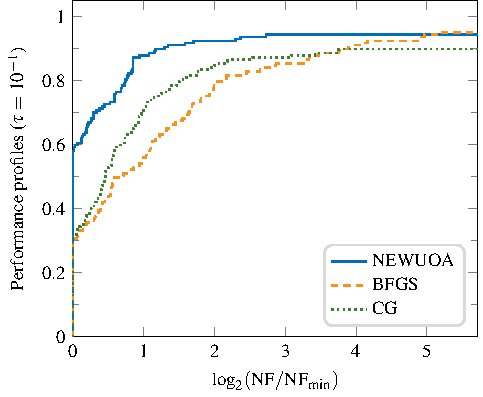
\includegraphics[width=\textwidth]{perf-plain-bfgs_cg_pdfo-50-1.pdf}
        \caption{$\sigma = 0$}
        \label{fig:ppu-fdiff-plain}
    \end{subfigure}
    \hfill
    \begin{subfigure}{.32\textwidth}
        \centering
        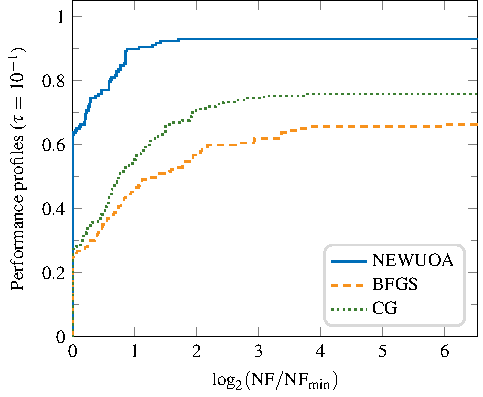
\includegraphics[width=\textwidth]{perf-noisy-bfgs_cg_pdfo-50-10-1.pdf}
        \caption{$\sigma = 10^{-10}$}
    \end{subfigure}
    \hfill
    \begin{subfigure}{.32\textwidth}
        \centering
        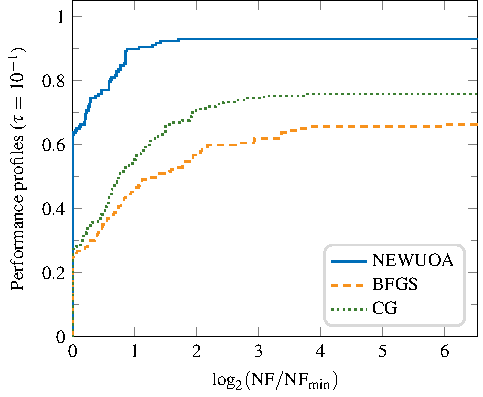
\includegraphics[width=\textwidth]{perf-noisy-bfgs_cg_pdfo-50-10-1.pdf}
        \caption{$\sigma = 10^{-10}$}
    \end{subfigure}
    \begin{subfigure}{.32\textwidth}
        \centering
        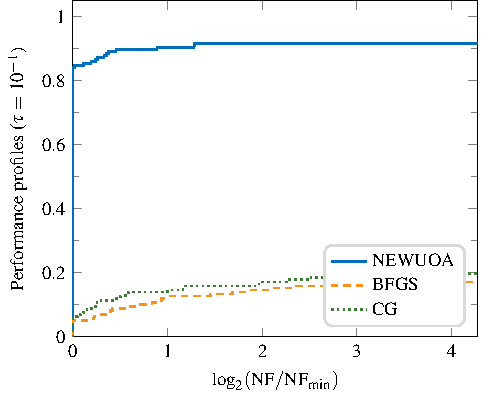
\includegraphics[width=\textwidth]{perf-noisy-bfgs_cg_pdfo-50-8-1.pdf}
        \caption{$\sigma = 0$}
    \end{subfigure}
    \hfill
    \begin{subfigure}{.32\textwidth}
        \centering
        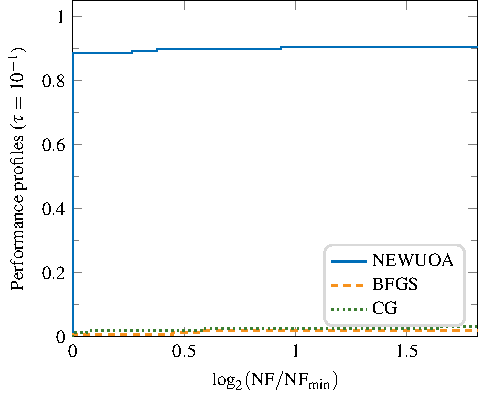
\includegraphics[width=\textwidth]{perf-noisy-bfgs_cg_pdfo-50-6-1.pdf}
        \caption{$\sigma = 10^{-10}$}
        \label{fig:ppu-fdiff-noisy-6}
    \end{subfigure}
    \hfill
    \begin{subfigure}{.32\textwidth}
        \centering
        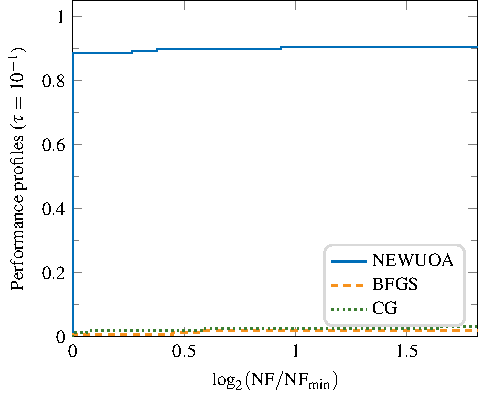
\includegraphics[width=\textwidth]{perf-noisy-bfgs_cg_pdfo-50-6-1.pdf}
        \caption{$\sigma = 10^{-8}$}
        \label{fig:ppu-fdiff-noisy-6}
    \end{subfigure}
    \caption{Performance profiles of \gls{newuoa}, \gls{bfgs}, and \gls{cg} on problems of dimension at most~$50$}
\end{figure}

Overall, on the noise-free problems, \gls{newuoa} is slightly more reliable than \gls{bfgs} and \gls{cg}.
Moreover, \gls{newuoa} evidently outperforms the two other solvers on noisy problems.
The performances of \gls{bfgs} and \gls{cg} deteriorate significantly when Gaussian noise is imposed as in~\eqref{eq:noisy-obj}, even though the noise level is not high and the convergence tolerance is not demanding.

Note that our results do not contradict the observations in~\cite{Shi_Etal_2022}, where the difference parameter~$h$ is chosen more carefully, according to the noise levels and the smoothness of the problems.
We rather keep the default value provided for the solvers \gls{bfgs} and \gls{cg} by SciPy~\cite{Virtanen_Etal_2020}.
As commented in~\cite{Shi_Etal_2022}, the performance of methods based on finite differences is encouraging when there is no noise, yet much more care is needed when the problems are noisy.
\Gls{newuoa} performs robustly with the noise according to this experiment, which agrees with the observations in~\cite{Shi_Etal_2022}.


\subsection{Comparison on the CUTEst library}

We now compare the performances of the Powell's \gls{dfo} methods for solving unconstrained problems.
To that end, we first repeat the previously described noise-free experiment.
Performance profiles on unconstrained problems of dimensions at most~$10$ and~$50$ are provided respectively in Figures~\ref{fig:ppu-10} and~\ref{fig:ppu-50}.
According to Figure~\ref{fig:ppu-10}, \gls{uobyqa} performs better than all the other solvers on small problems.
This can be explained by the fact that it uses quadratic models obtained by fully-determined interpolation.
However, we excluded \gls{uobyqa} from the second experiment, because the execution time was excessively long on problems with moderately high dimensions, due to the fully-determined interpolation that it does.
Moreover, \gls{cobyla} is always outperformed by all other solvers.
This is because it uses only linear models to approximate the objective and constraint functions of the problems, which are not as precise as the quadratic models employed by other solvers.

\begin{figure}[ht]
    \begin{subfigure}{.48\textwidth}
        \centering
        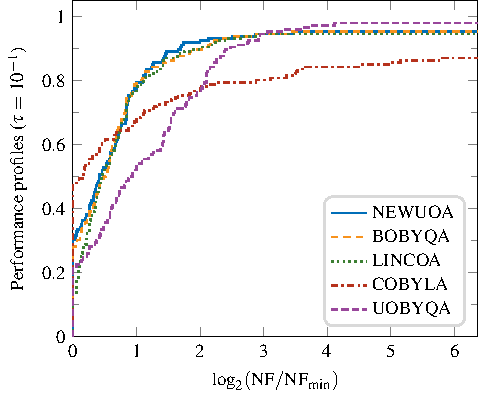
\includegraphics[width=\textwidth]{perf-plain-pdfo-10-1.pdf}
        \caption{Dimension at most~$10$.}
        \label{fig:ppu-10}
    \end{subfigure}
    \hfill
    \begin{subfigure}{.48\textwidth}
        \centering
        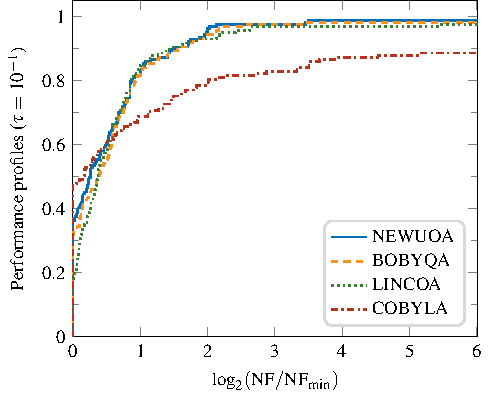
\includegraphics[width=\textwidth]{perf-plain-pdfo-50-1.pdf}
        \caption{Dimension at most~$50$.}
        \label{fig:ppu-50}
    \end{subfigure}
    \caption{Performance profile of Powell's \glsfmtshort{dfo} solvers}
\end{figure}

Consider however the previously detailed noisy experiment, applied to Powell's \gls{dfo} solvers.
Figure~\ref{fig:ppun-50} presents the performance profiles on the same unconstrained problems of dimension at most~$50$ from the CUTEst library as the previous experiment by randomizing the objective functions with~$\sigma = 10^{-2}$.

\begin{figure}[ht]
    \centering
    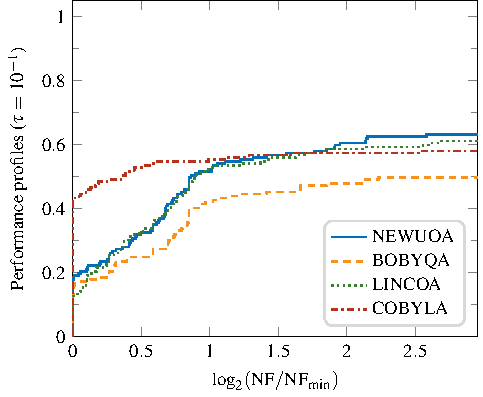
\includegraphics[width=.48\textwidth]{perf-noisy-pdfo-50-2-1.pdf}
    \caption{Performance profile of Powell's \glsfmtshort{dfo} solvers on noisy problems of dimension at most~$50$}
    \label{fig:ppun-50}
\end{figure}

It is interesting to observe the performance of \gls{cobyla} in this experiment.
Even though it is not particularly designed for such kind of problems and uses the simplest models, we observe that \gls{cobyla} defeats all other solvers on unconstrained problems, for~$\tau = 10^{-1}$.
It seems that the linear models of \gls{cobyla} are more robust to noise, but we have not yet derived a theory for this behavior.

\subsection{An example of hyperparameter tuning problem}

We now consider the more practical problem of the hyperparameter tuning of a \gls{svm}.
The model we consider is a~$C$-SVC~\cite{Chang_Lin_2011} for binary classification problems with an \gls{rbf} kernel, admitting two hyperparameters: a regularization parameter~$C > 0$ and a kernel coefficient~$\gamma > 0$.
We compare \gls{pdfo} with \gls{tpe} and \gls{rs}, two standard solvers
in the Python package \texttt{hyperopt}~\cite{Bergstra_Yamins_Cox_2013} for hyperparameter tuning.
Our experiments are based on binary classifications problems from the LIBSVM datasets\footnote{\url{https://www.csie.ntu.edu.tw/~cjlin/libsvmtools/datasets/}.}.
A description of the datasets employed is provided in Table~\ref{tab:htdata}.

\begin{table}[ht]
    \caption{Considered LIBSVM dataset descriptions}
    \label{tab:htdata}
    \centering
    \begin{tabular}{cS[table-format=2]S[table-format=5]}
        \toprule
        Dataset~$\mathcal{P}$   & {Dimension}   & {Dataset size}\\
        \midrule
        splice                  & 60            & 1000\\
        svmguide1               & 4             & 3088\\
        ijcnn1                  & 22            & 49990\\
        \bottomrule
    \end{tabular}
\end{table}

A dataset~$\mathcal{P}$ is divided into two disjoint parts: a training dataset~$\mathcal{L}$ and a testing dataset~$\mathcal{T}$, with~$\mathcal{P} = \mathcal{L} \cup \mathcal{T}$.

The problem we consider is as follows.
We want to maximize the~$5$-fold \gls{auc} validation score of the \gls{svm} trained on~$\mathcal{L}$ with respect to the hyperparameters~$C$ and~$\gamma$.
The \gls{auc} score, a real number in~$[0, 1]$, measures the area underneath the \gls{roc} curve, a graph representing the performance of a binary classification model.
This curve plots the true positive classification rate with respect to the false positive classification rate at different classification thresholds.
The~$5$-fold \gls{auc} validation score corresponds to the following.
The set~$\mathcal{L}$ is split into~$5$ folds, and the model is trained~$5$ times, on each union of~$4$ distinct folds.
After each training, the \gls{auc} score is calculated on the remaining fold, which was not involved in the training process, giving rise to~$5$ \gls{auc} scores, the average of which corresponds to the~$5$-fold \gls{auc} validation score.

The numerical results for this experiment are provided in Tables~\ref{tab:splice}--\ref{tab:ijcnn1}.
The \gls{auc} scores and accuracies presented in the tables correspond to the ones computed on~$\mathcal{T}$ using an \gls{svm} trained on~$\mathcal{L}$, with the tuned parameters~$C$ and~$\gamma$.

In terms of \gls{auc} score and accuracy, we observe that \gls{pdfo} achieved a clearly better result than \gls{tpe} and \gls{rs} on the ``splice'' dataset, and they all attain comparable results on all the other datasets.
However, \gls{pdfo} always uses much less function evaluations, and hence, much less computation time.
The difference in the computation time is particularly visible on the dataset ``ijcnn1'' in Table~\ref{tab:ijcnn1}, as the size of this dataset is large, so that each function evaluation takes much time.
In summary, we can conclude that \gls{pdfo} performs better than \gls{tpe} and \gls{rs} on these problems.

\begin{table}[!ht]
    \caption{Hyperparameter tuning problem on the dataset ``splice.''}
    \label{tab:splice}
    \centering
    \begin{tabular}{cSSS[table-format=3]S}
        \toprule
        Solver      & {AUC Score ($10^{-1}$)}   & {Accuracy ($10^{-1}$)}    & {No.\ eval}   & {Exec.\ time (\si{\second})}\\
        \midrule
        \Gls{pdfo}  & 9.27                      & 7.37                      & 33            & 5.11\\
        \Gls{rs}    & 5.00                      & 5.20                      & 100           & 8.23\\
        \Gls{rs}    & 5.00                      & 5.20                      & 200           & 16.15\\
        \Gls{rs}    & 5.00                      & 5.20                      & 300           & 24.73\\
        \Gls{tpe}   & 5.00                      & 5.20                      & 100           & 8.22\\
        \Gls{tpe}   & 5.00                      & 5.20                      & 300           & 23.57\\
        \bottomrule
    \end{tabular}
\end{table}

\begin{table}[!ht]
    \caption{Hyperparameter tuning problem on the dataset ``svmguide1.''}
    \centering
    \begin{tabular}{cS[table-format=3]SSS}
        \toprule
        Solver      & {AUC Score ($10^{-1}$)}   & {Accuracy ($10^{-1}$)}    & {No.\ eval.}  & {Exec.\ time (\si{\second})}\\
        \midrule
        \Gls{pdfo}  & 9.95                      & 9.66                      & 51            & 2.83\\
        \Gls{rs}    & 9.94                      & 9.61                      & 100           & 10.22\\
        \Gls{rs}    & 9.95                      & 9.67                      & 200           & 20.51\\
        \Gls{rs}    & 9.95                      & 9.68                      & 300           & 30.75\\
        \Gls{tpe}   & 9.95                      & 9.65                      & 100           & 8.65\\
        \Gls{tpe}   & 9.95                      & 9.68                      & 300           & 22.38\\
        \bottomrule
    \end{tabular}
\end{table}

\begin{table}[!ht]
    \caption{Hyperparameter tuning problem on the dataset ``ijcnn1.''}
    \label{tab:ijcnn1}
    \centering
    \begin{tabular}{cS[table-format=3]SSS}
        \toprule
        Solver      & {AUC Score ($10^{-1}$)}   & {Accuracy ($10^{-1}$)}    & {No.\ eval.}  & {Exec.\ time (\SI{}[10^3]{\second})}\\
        \midrule
        \Gls{pdfo}  & 9.97                      & 9.80                      & 44            & 2.48\\
        \Gls{rs}    & 9.97                      & 9.82                      & 100           & 3.99\\
        \Gls{rs}    & 9.98                      & 9.77                      & 200           & 7.60\\
        \Gls{rs}    & 9.97                      & 9.77                      & 300           & 11.52\\
        \Gls{tpe}   & 9.98                      & 9.79                      & 100           & 3.42\\
        \Gls{tpe}   & 9.98                      & 9.79                      & 300           & 8.81\\
        \bottomrule
    \end{tabular}
\end{table}
\section{Conclusions}
\label{sec:conclude}

We have presented the package \gls{pdfo} for Python and MATLAB, which aims at simplifying the use of the Powell's \gls{dfo} solvers.
More information about the package itself can be found on the \gls{pdfo} website~(\url{https://www.pdfo.net/}), together with different examples of use.
The scope of \gls{pdfo} in the future is not limited only to the Powell's \gls{dfo} solvers.
For instance, the authors are currently working on a new solver for nonlinearly constrained optimization, named \gls{cobyqa}~\cite{Ragonneau_2022}.
It is aimed to be added to \gls{pdfo}, and other \gls{dfo} solvers may be included in the future.

\section{Statements and declarations}

\subsection{Funding}

This work was funded by the University Grants Committee of Hong Kong under the
projects PF18-24698 (Hong Kong Ph.D.~Fellowship Scheme), PolyU 253012/17P, PolyU 153054/20P,
and PolyU 153066/21P.
It was also supported by The Hong Kong Polytechnic University under project P0009767.

\subsection{Competing interests}

The authors have no relevant financial or non-financial interests to disclose.

\subsection{Data availability}

The source code of the \gls{pdfo} package is available at \mbox{\url{https://www.pdfo.net/}}.
The source code of the numerical experiments presented in this manuscript is available at
\mbox{\url{https://www.github.com/pdfo/paper/blob/main/experiments/}}.

\bibliographystyle{spmpsci}
\bibliography{pdfo}

\end{document}
